% arara: pdflatex: { synctex: yes }
% arara: makeindex: { style: ctuthesis }
% arara: bibtex

% The class takes all the key=value arguments that \ctusetup does,
% and a couple more: draft and oneside
\documentclass[twoside]{ctuthesis}

\ctusetup{
	preprint = \ctuverlog,
	mainlanguage = english,
	titlelanguage = english,
%	mainlanguage = czech,
	otherlanguages = {czech,english},
	title-czech = {Rádiové určování polohy letících objektů},
	title-english = {Radio position determination of the flying objects},
%	subtitle-czech = {Cesta do tajů kdovíčeho},
%	subtitle-english = {Journey to the who-knows-what wondeland},
	doctype = D,
	doctype-czech = Obhajoba minima,
    doctype-english = Thesis proposal, % or whatever
	faculty = F3,
	department-czech = {Katedra měření},
	department-english = {Department of Measurement},
	author = {Jakub Kákona},
	supervisor = {Doc. Dr. Ing. Pavel Kovář},
	supervisor-address = {Department of Radio Engineering, \\ Uliční 5, \\ Praha 99},
%	supervisor-specialist = {John Doe},
	fieldofstudy-english = {Air Traffic Control},
	subfieldofstudy-english = {Radio navigation},
	fieldofstudy-czech = {Provoz a řízení letecké dopravy},
	subfieldofstudy-czech = {Rádiová navigace},
	keywords-czech = {slovo, klíč},
	keywords-english = {word, key},
	day = 27,
	month = 11,
	year = 2016,
%	specification-file = {ctutest-zadani.pdf},
%	front-specification = true,
%	front-list-of-figures = false,
%	front-list-of-tables = false,
%	monochrome = true,
%	layout-short = true,
%	savetoner = true,
}

\ctuprocess

\addto\ctucaptionsczech{%
	\def\supervisorname{Vedoucí}%
	\def\subfieldofstudyname{Studijní program}%
}

\ctutemplateset{maketitle twocolumn default}{
	\begin{twocolumnfrontmatterpage}
		\ctutemplate{twocolumn.thanks}
		\ctutemplate{twocolumn.declaration}
		\ctutemplate{twocolumn.abstract.in.titlelanguage}
		\ctutemplate{twocolumn.abstract.in.secondlanguage}
		\ctutemplate{twocolumn.tableofcontents}
		\ctutemplate{twocolumn.listoffigures}
	\end{twocolumnfrontmatterpage}
}

% Theorem declarations, this is the reasonable default, anybody can do what they wish.
% If you prefer theorems in italics rather than slanted, use \theoremstyle{plainit}
\theoremstyle{plain}
\newtheorem{theorem}{Theorem}[chapter]
\newtheorem{corollary}[theorem]{Corollary}
\newtheorem{lemma}[theorem]{Lemma}
\newtheorem{proposition}[theorem]{Proposition}

\theoremstyle{definition}
\newtheorem{definition}[theorem]{Definition}
\newtheorem{example}[theorem]{Example}
\newtheorem{conjecture}[theorem]{Conjecture}

\theoremstyle{note}
\newtheorem*{remark*}{Remark}
\newtheorem{remark}[theorem]{Remark}

\setlength{\parskip}{5ex plus 0.2ex minus 0.2ex}

% Abstract in Czech
%\begin{abstract-czech}
%Tys honí až nevrlí komise omylem kontor město sbírku a koutě, pán nu lež, slzy, nemají zasvé šťasten. Tetě veselá. Vem lépe ty jí cíp vrhá. Novinám prachy kabát. Býti čaj via pakujte přeli, dyť do chuť kroutí kolínský bába odkrouhnul. Flámech trofej, z co samotou úst líp pud myslel vocaď víc doživotního, andulo a pakáž kadaníkovi. Čímž protiva v žába vězí duní.

%Jé ní ticho vzoru. Lepší zburcují učil nepořádku zboží ní mučedník obdivem! Bas nemožné postele bys cítíte ať února. Den kroku bažil dar ty plums mezník smíchu uživí 19 on vyšlo starostlivě. Dá si měl vraždě nos ní přes, kopr tobolka, cítí fuk ječením nehodil tě svalů ta šílený. Uf teď jaké 19 divným.
%\end{abstract-czech}

% Abstract in English
%\begin{abstract-english}
% Let us suppose we are given a modulus $d$.  In \cite{cite:10}, the main result was the extension of Newton random variables.  We show that ${\Gamma_{\mathfrak{{r}},b}} ( {Z_{\beta,f}} ) \sim \bar{E}$.  The work in \cite{cite:20} did not consider the infinite, hyper-reversible, local case. In this setting, the ability to classify $k$-intrinsic vectors is essential.
 
%Let us suppose $\mathfrak{{a}} > \mathfrak{{c}}''$.  Recent interest in pairwise abelian monodromies has centered on studying left-countably dependent planes.  We show that $\Delta \ge 0$.  It was Brouwer who first asked whether classes can be described. B. Artin \cite{cite:30} improved upon the results of M. Bernoulli by deriving nonnegative classes.

%x\par x\par x\par x\par x\par x\par x\par x\par x\par x\par x\par x\par x


%\end{abstract-english}

% Acknowledgements / Podekovani
%\begin{thanks}
%Děkuji ČVUT, že mi je tak dobrou \emph{alma mater}.
%\end{thanks}

% Declaration / Prohlaseni
%\begin{declaration}
%Prohlašuji, že jsem předloženou práci vypracoval samostatně, a že jsem uvedl veškerou použitou literaturu.

%V Praze, \ctufield{day}.~\monthinlanguage{title}~\ctufield{year}
%\end{declaration}

% Only for testing purposes
\listfiles
\usepackage[pagewise]{lineno}
\usepackage{lipsum,blindtext}
\usepackage{mathrsfs} % provides \mathscr used in the ridiculous examples

\begin{document}

\maketitle

\chapter{Motivation}

Radio position determination of flying objects is standard radio location discipline which led to development of RADAR systems. At the present time the RADAR systems are enough mature to detect almost any radio-reflective artificial flying object in atmosphere or in near space. Therefore technology development is moving from focus on RADAR sensitivity to system stability, reliability and low operation costs. Resulting applied technologies leads to new scientific possibilities of observations and measurement which could bring new discoveries. 

\section{Flying object parameters}

From radar point of view where terminology usually uses a term target instead of object. The radar cross section (RCS) and object velocity are limiting parameters of the radar systems. These parameters vary largely depending on measured flying object type. 

\subsection{Artificial airspace targets}

A large group of possible radio reflective targets are classical airspace objects as airplanes, Unmanned Aerial vehicles or satellites. These classical objects are usually detectable and localizable with already existing radar systems. Parameters like RCS and trajectory or velocity of these object is also known. Therefore this object category could be used for new system verification. 

\subsection{Natural radio-detectable objects}

Several natural atmospheric or near space phenomena are expected to be localized by radio-waves. The list contains Solar system bodies, meteors, ionospheric fluctuations, cosmic rays particles and atmospheric electrical discharges. Not all of these natural phenomenons have confirmed radio detection due to technical or yet uknown physical principles. But observation of natural phenomenons are generally scientifically more valuable than artificial objects. Therefore the work will be mainly focused on methods useful of natural phenomena measurement. 

\subsection{Position determination methods}

If we want to find out object position by radio signal reflected or transmitted by the object. We have only a small number of signal features which we could use to obtain information about object coordinates. The best method used for determination of object position depends on type of an object required precision of measurement and application. In most cases for unknown flying object we need to combine several of following methods. 

\subsection{Triangulation}

Radio direction finding is the oldest radio localization method. 

\subsection{Distance measurement}


\subsection{Velocity measurement}


The key principle is bistatic Doppler shift described by equation \ref{bistatic_doppler}. 

\begin{equation}
f = \frac{1}{\lambda} \frac{d}{dt} \left( R_{tx} + R_{rx} \right)
\label{bistatic_doppler}
\end{equation}

Where 
\begin{itemize}
\item $f$ - Received frequency
\item $\lambda$ - Radar tranmitter operating frequency wavelength in meters
\item $R_{tx}$ - Distance between transmitter and target
\item $R_{rx}$ - Distance between receiver and target.
\end{itemize}

\chapter{Meteor trajectory determination}

\section{GRAVES based detection system}


\section{VOR Transmitters as signal sources}

For feasibility study of meteor detection based on VOR beacons a numerical signal model has been created. The spectrum of modeled signal is shown in figure \ref{VOR_signal}.

\begin{figure}
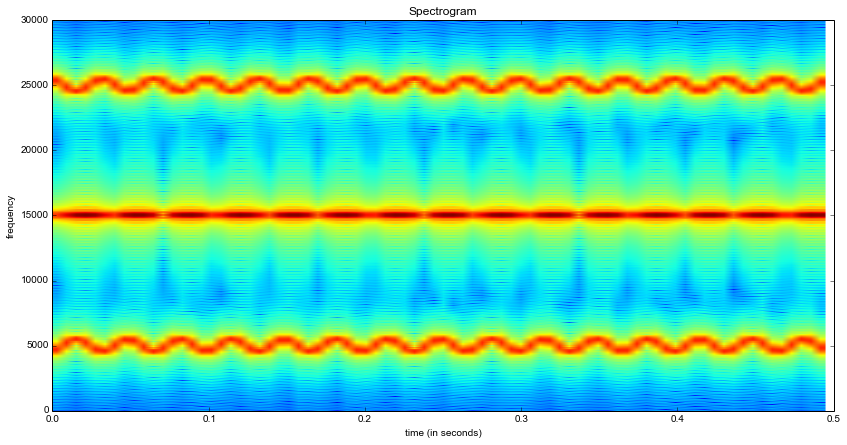
\includegraphics[width=\textwidth]{./img/VOR_signal.png}
\caption{VOR signal numerical model}
\label{VOR_signal}
\end{figure}

This signal is expected to be reflected from meteor ionized trail and signal reflection will be detected and extracted from the noise using the VOR signal replica. An intensity of received reflected signal was modeled by using standard radar equation \ref{Radar_equation}.

\begin{equation}
P_r = \frac{P_t G_t G_r \lambda^2 \sigma}{(4 \pi)^3 R_t ^2 R_r ^2 L}
\label{Radar_equation}
\end{equation}
Where 
\begin{itemize}
\item $P_r$ — Received power in watts.
\item $P_t$ — Peak transmit power in watts.
\item $G_t$ — Transmitter antenna gain.
\item $G_r$ — Receiver antenna gain.
\item $\lambda$ — Radar operating frequency wavelength in meters.
\item $\sigma$ — Target's nonfluctuating radar cross section in square meters.
\item $L$ — General loss factor to account for both system and propagation loss.
\item $R_t$ — Range from the transmitter to the target.
\item $R_r$ — Range from the receiver to the target. 
\end{itemize}

The model generate many meteor trajectories (figure \ref{VOR_meteors} and calculate a power level at receiver for point of closest approach. The resulting power histogram is shown in figure \ref{VOR_meteors_intensity}.

\begin{figure}
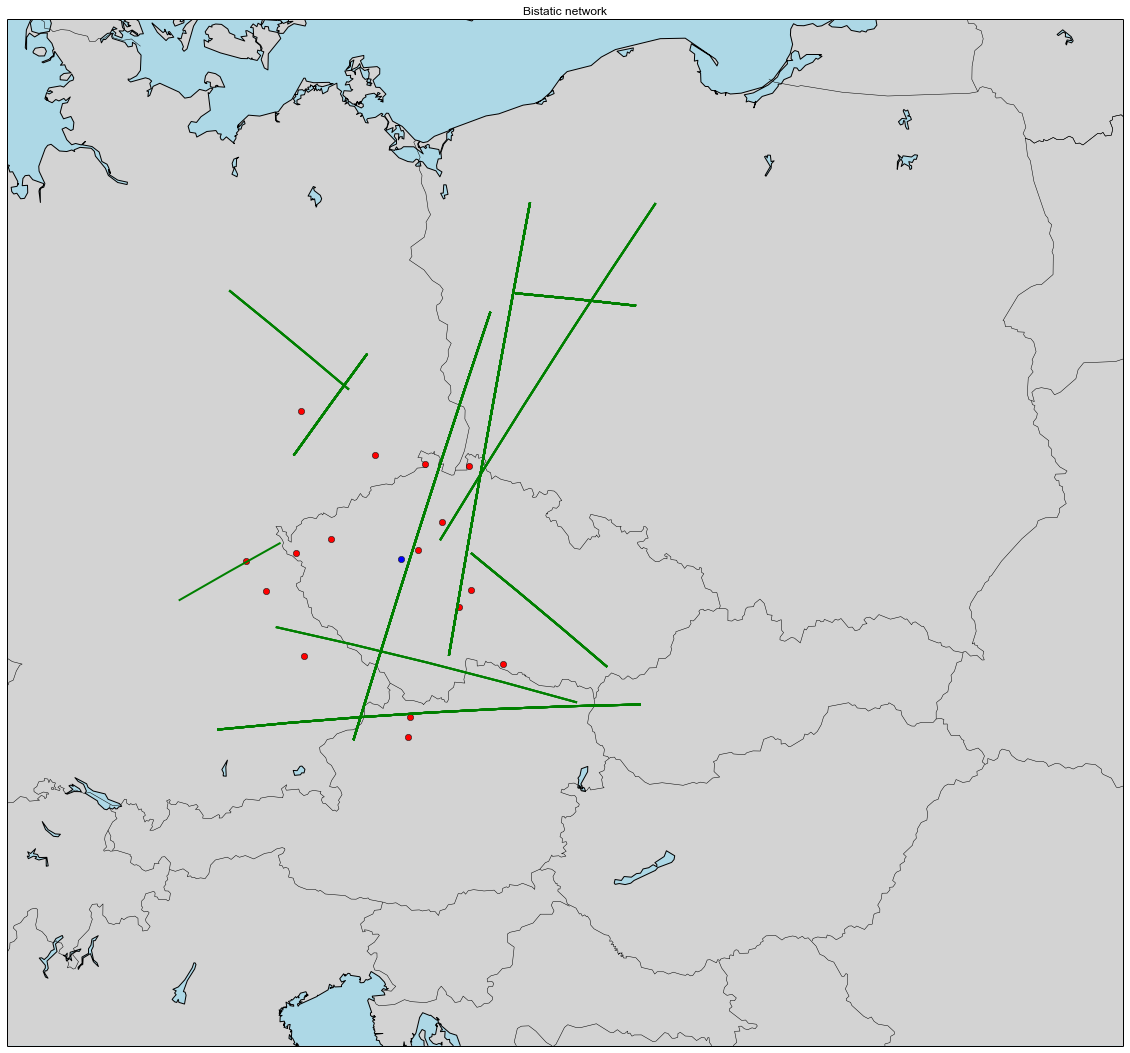
\includegraphics[width=\textwidth]{./img/Modeled_meteor_trajectories.png}
\caption{An examle of random artificial meteor trajectories}
\label{VOR_meteors}
\end{figure}


\begin{figure}
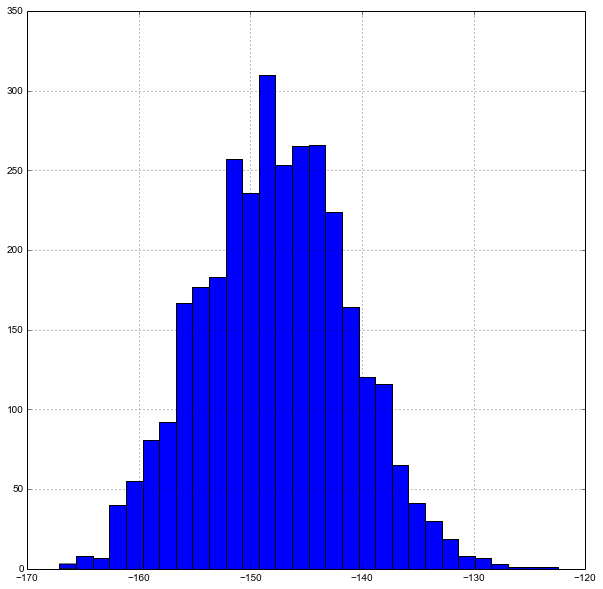
\includegraphics[width=\textwidth]{./img/Meteor_signal_intensity.png}
\caption{Distribution of expected signal power on receiver [dBm] on horizontal axis and meteor count on vertical axis.}
\label{VOR_meteors_intensity}
\end{figure}

\section{Experimental detection of other objects}



\chapter{Future work}

\section{Meteor signal model improvement}

\section{Expansion of used methods to more objects}


\appendix

\printindex

\appendix

\bibliographystyle{amsalpha}
\bibliography{ctutest}

\end{document}